\documentclass{standalone}
\usepackage{tikz}
\usepackage{ctex,siunitx,ninecolors}
\setCJKmainfont{Noto Serif CJK SC}
\usepackage{tkz-euclide}
\usepackage{amsmath}
\usetikzlibrary{patterns, calc}
\usetikzlibrary {decorations.pathmorphing, decorations.pathreplacing, decorations.shapes}
\begin{document}
\small
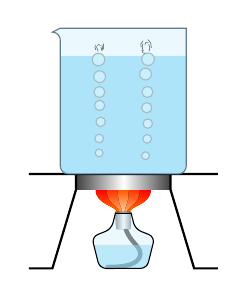
\begin{tikzpicture}[>=latex,scale=1.0]
  % \useasboundingbox(-1.4,-1.4)rectangle(1.4,1.4);
  \fill[top color=red,bottom color=orange](-0.35,1)..controls(-0.35,0.8)and(-0.075,0.8)..(-0.075,0.7)--(0.075,0.7)..controls(0.075,0.8)and(0.35,0.8)..(0.35,1);
  \fill[top color=red!60!orange,bottom color=orange!60](-0.21,1)..controls(-0.21,0.8)and(-0.045,0.8)..(-0.045,0.7)--(0.045,0.7)..controls(0.045,0.8)and(0.21,0.8)..(0.21,1);
  \fill[top color=red!30!orange,bottom color=orange!30](-0.07,1)..controls(-0.07,0.8)and(-0.015,0.8)..(-0.015,0.7)--(0.015,0.7)..controls(0.015,0.8)and(0.07,0.8)..(0.07,1);
  \draw[ultra thick,darkgray]( 0.000,0.700)..controls( 0.000,0.300)and( 0.296,0.300)..( 0.197,0.123)..controls( 0.136,0.032)and(-0.021,0.017)..(-0.222,0.018);
  \fill[rounded corners=0.8mm,cyan!60,opacity=0.5](-0.375,0.3)--(-0.3,0)--(0.3,0)--(0.375,0.3);
  \fill[left color=gray,right color=gray,middle color=white](-0.1010,0.72)--(-0.09,0.5)--(0.09,0.5)--(0.1010,0.72);
  \draw[rounded corners=0.8mm,fill=cyan!20,fill opacity=0.4](-0.1,0.7)--(-0.15,0.5)--(-0.4,0.4)--(-0.3,0)--(0.3,0)--(0.4,0.4)--(0.15,0.5)[sharp corners]--(0.1,0.7)--cycle;

  \fill[left color=darkgray,right color=darkgray,middle color=white](-0.6,1.2)rectangle(0.6,1.0);
  \draw[thick](-1.2,1.2)--(1.2,1.2)(-0.6,1.2)--(-0.6,1.0)--(-0.9,0)--(-1.2,0)(0.6,1.2)--(0.6,1.0)--(0.9,0)--(1.2,0);
  \fill[cyan!40!white](-0.8,2.7)--(-0.8,1.3)arc(-180:-90:0.1)--(0.7,1.2)arc(-90:0:0.1)--(0.8,2.7);
  \foreach \y[count =\i] in {1.45,1.65,...,2.65}
  {
    \fill[cyan!20!white,draw=cyan!20!gray](-0.3+0.02*rand,\y+0.02*rand)circle(0.045+0.005*\i);
    \fill[cyan!20!white,draw=cyan!20!gray](0.3+0.02*rand,\y+0.02*rand)circle(0.045+0.005*\i);
  }
  \draw[very thin] (-0.349,2.776)..controls(-0.365,2.794)and(-0.359,2.817)..(-0.353,2.838)
  (-0.318,2.755)..controls(-0.318,2.789)and(-0.349,2.794)..(-0.340,2.821)
  (-0.331,2.831)..controls(-0.319,2.848)and(-0.309,2.845)..(-0.289,2.831)
  (-0.281,2.764)..controls(-0.276,2.780)and(-0.275,2.800)..(-0.285,2.814)
  (-0.267,2.783)..controls(-0.262,2.807)and(-0.263,2.823)..(-0.272,2.836)
  (-0.253,2.856)..controls(-0.241,2.821)and(-0.249,2.784)..(-0.263,2.767)
  (0.227,2.806)..controls(0.209,2.843)and(0.224,2.865)..(0.253,2.890)
(0.255,2.762)..controls(0.235,2.804)and(0.241,2.823)..(0.250,2.857)
(0.235,2.769)..controls(0.241,2.736)and(0.261,2.726)..(0.278,2.730)
(0.273,2.841)..controls(0.277,2.875)and(0.295,2.879)..(0.318,2.869)
(0.324,2.849)..controls(0.343,2.817)and(0.340,2.785)..(0.329,2.759)
(0.313,2.906)..controls(0.348,2.875)and(0.359,2.842)..(0.357,2.802);
  \draw[cyan!30!darkgray,fill=cyan!20,fill opacity=0.4](-0.9,3.0)arc(90:0:0.1)--(-0.8,1.3)arc(-180:-90:0.1)--(0.7,1.2)arc(-90:0:0.1)--(0.8,3.05)--(-0.8,3.05)--cycle;
  
 
\end{tikzpicture}
\end{document}